\section{Results}\label{sec:results}
\subsection{Filtered density fields}
Fig.~\ref{fig:slices} compares line-of-sight and transverse slices of the smoothed density field. The noFG field contains interconnected overdense structures and extended underdense regions. After the horizontal cut, the line-of-sight slices develop bands extending in the transverse ($x$ or $y$) direction, with more rapid alternation along the line of sight. Removing low $|k_\parallel|$ suppresses slowly varying radial structure; Gaussian smoothing then favours the surviving modes with relatively small $k_\perp$, producing this transverse coherence. These bands are an imprint of the filter, not additional matter sheets formed by gravitational evolution.

At both displayed redshifts, the horizontal cut reduces the three-dimensional standard deviation from about 0.26 to 0.012. Each panel is normalized by its own field standard deviation, so its colour contrast does not represent the absolute fluctuation amplitude. The $m=0.294$ field remains visually close to the horizontal-cut field, whereas the stronger wedge alters the transverse pattern and further reduces the variance. This follows the mask geometry in Fig.~\ref{fig:foregroundmask}: the weak wedge first adds removal at $k_\perp>0.1/0.294\simeq0.34\,h\,\mathrm{Mpc}^{-1}$, where $R=20\,h^{-1}\mathrm{Mpc}$ smoothing is already severe.

\begin{figure*}
\centering
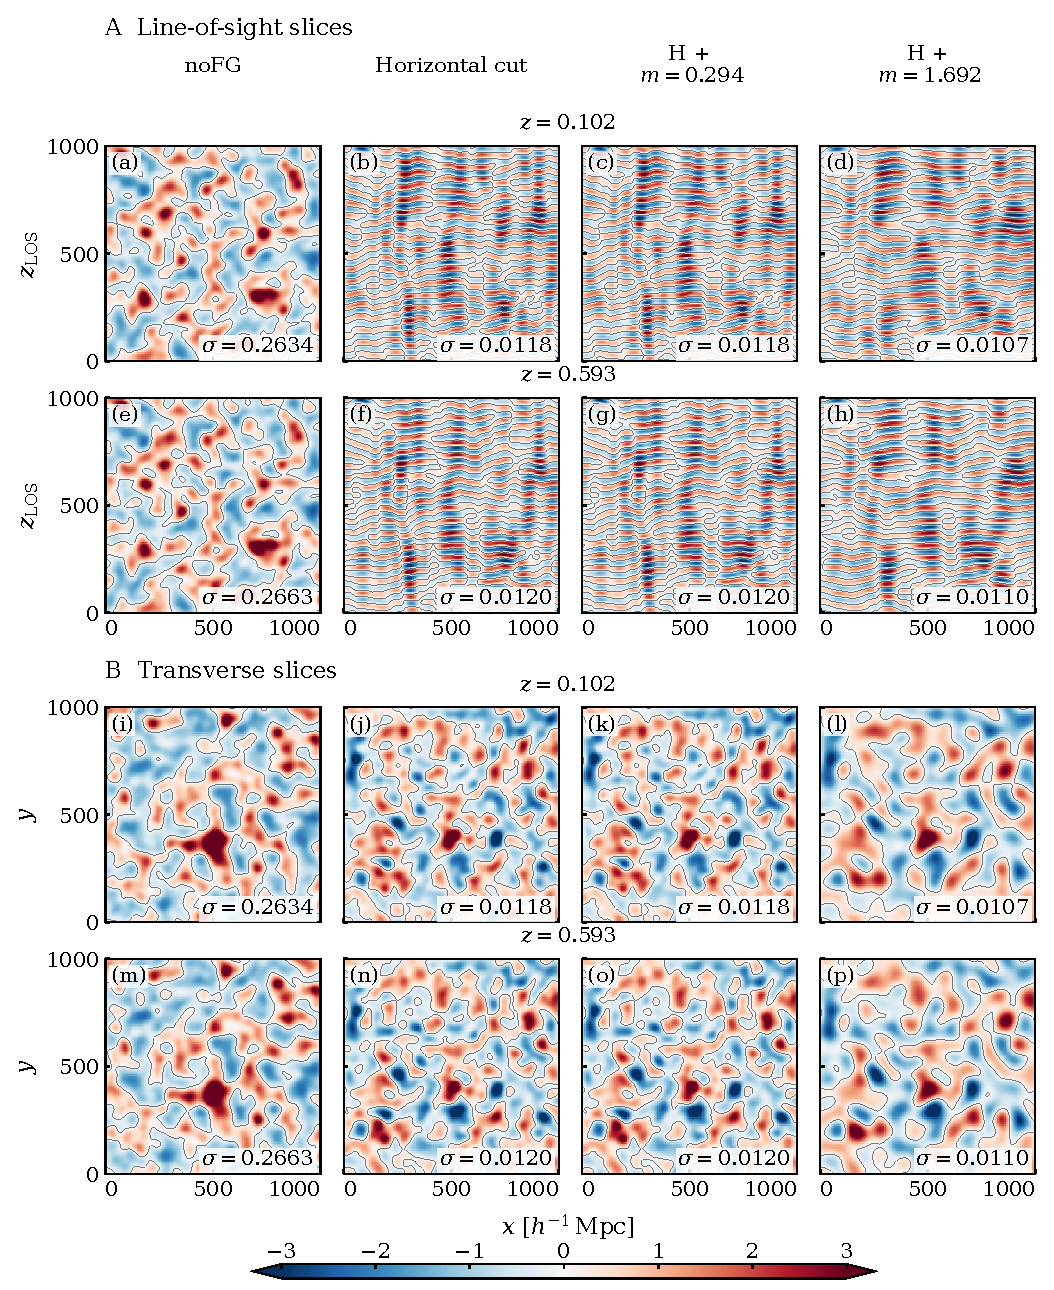
\includegraphics[width=.98\textwidth]{figures/fig__slices.pdf}
\caption{Smoothed H\,I density field in the simulation cosmology at $z=0.102$ and 0.593, normalized by its standard deviation $\sigma_{\rm 3D}$ (labelled $\sigma$ in each panel). A: line-of-sight slices at $y=498\,h^{-1}\mathrm{Mpc}$; B: transverse slices at $z_{\rm LOS}=498\,h^{-1}\mathrm{Mpc}$. Contours mark the median of each three-dimensional field; the colour scale is $\delta_{\rm filtered}/\sigma_{\rm 3D}$, clipped at $\pm3$. All spatial coordinates are in $h^{-1}\mathrm{Mpc}$.}\label{fig:slices}
\end{figure*}

\subsection{Genus curves and intrinsic evolution}
Fig.~\ref{fig:foregroundcurves} shows how foreground removal changes the genus curve at $z=0.102$. The horizontal cut raises the fitted amplitude by about a factor of 4.6, while the strong wedge reduces it relative to the horizontal-cut case. The lower field variance in Fig.~\ref{fig:slices} does not imply a lower genus amplitude: at fixed volume fraction, genus measures connectivity rather than the absolute density contrast. Selective mode removal changes characteristic spatial scales and directional coherence, so it can change the number of tunnels and disconnected regions per unit volume even while suppressing fluctuations. In Gaussian-field theory the amplitude depends on normalized field gradients and their anisotropy \citep{Matsubara1996IsodensityRedshift}; this provides a qualitative interpretation, not a prediction of the measured factor of 4.6.

The weakest wedge ($m\simeq0.294$) matches the displayed horizontal-cut curve because the additional removed modes are strongly suppressed by Gaussian smoothing (Fig.~\ref{fig:foregroundmask}). A stronger wedge reaches modes that survive the smoothing and changes the transverse coherence, consistent with the lower amplitude in Fig.~\ref{fig:foregroundcurves}. The horizontal-cut and weakest-wedge joint statistics agree at 1284 of the 1285 scan points.

\begin{figure}
\centering
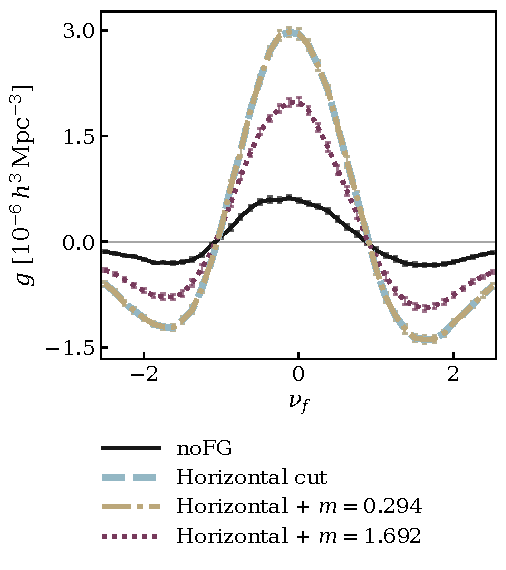
\includegraphics[width=\columnwidth]{figures/fig__noFG_hcut_msan_comp.pdf}
\caption{Genus curves at $z=0.102$ in the simulation cosmology for the four foreground treatments. Error bars are from the 64-block fixed-field jackknife estimate.}\label{fig:foregroundcurves}
\end{figure}

Fig.~\ref{fig:redshifts} separates the nearly overlapping genus curves in its upper row from their small redshift differences below. In the simulation cosmology, the curves change little between $z=0.10$ and 0.59, but the lower panels retain the threshold dependence needed to define $\boldsymbol I_i$. A common growth of the density amplitude alone would cancel at fixed volume fraction; the remaining evolution can reflect nonlinear growth, tracer selection and redshift-space effects, whose individual contributions are not separated here. Table~\ref{tab:amplitudes} lists all three higher-redshift changes relative to $z_1=0.10235$, separately for each sample and foreground treatment. Without foreground cuts, the endpoint fitted amplitude changes by $+0.11$ per cent for the top-$10^6$ sample and $+2.9$ per cent for the full valid catalogue. These changes are descriptive, not significance estimates: their uncertainties require cross-redshift covariance. For the horizontal-cut top-$10^6$ sample, the intermediate snapshots differ from the lowest-redshift amplitude by $-1.44$ and $-1.40$ per cent, although the endpoint difference is only $+0.25$ per cent. Thus a small endpoint change does not imply negligible evolution throughout the interval. The analysis below uses the full curves rather than the fitted amplitudes.

\begin{table*}
\centering
\caption{Redshift evolution of the fitted genus amplitude in the simulation cosmology. Entries give $100[A(z)/A(z_1)-1]$ in per cent, with $z_1=0.10235$ as the reference for each sample and foreground treatment. The reference change is zero by definition. Values are rounded to two decimal places; they are descriptive changes, not significance estimates.}
\label{tab:amplitudes}
\begin{tabular}{@{}lrrrrrr@{}}
\toprule
& \multicolumn{3}{c}{Top $10^6$} & \multicolumn{3}{c}{All valid objects} \\
\cmidrule(lr){2-4}\cmidrule(l){5-7}
Filter & $z=0.19095$ & $z=0.31970$ & $z=0.59339$ & $z=0.19095$ & $z=0.31970$ & $z=0.59339$ \\
\midrule
noFG & $+0.01$ & $-0.25$ & $+0.11$ & $+0.45$ & $+1.18$ & $+2.91$ \\
Horizontal cut & $-1.44$ & $-1.40$ & $+0.25$ & $-0.20$ & $-0.30$ & $-0.48$ \\
Horizontal + $m=0.294$ & $-1.44$ & $-1.40$ & $+0.25$ & $-0.20$ & $-0.30$ & $-0.48$ \\
Horizontal + $m=1.692$ & $-1.31$ & $-1.54$ & $+0.22$ & $0.00$ & $+0.17$ & $+0.10$ \\
\bottomrule
\end{tabular}
\end{table*}



\subsection{Cosmological Dependence}
Fig.~\ref{fig:cosmologies} compares the genus at $z=0.593$ under the simulation cosmology and two illustrative distance--redshift relations. The lower panels reveal differences that are less apparent in the overlapping curves above. With smoothing and foreground cuts fixed in scan coordinates, an AP remapping changes their physical scale and direction dependence, as well as the volume used to report genus density. The resulting differences therefore describe the response of this measurement procedure to the assumed cosmology.

Fig.~\ref{fig:covariance} shows how the redshift-difference measurements are weighted. Its diagonal blocks describe correlations between thresholds within a redshift pair, and its off-diagonal blocks describe correlations between pairs that share the same reference snapshot. The patterns change with foreground treatment, so the significance assigned to a residual depends on its shape relative to the covariance, not only on its visible amplitude.

Fig.~\ref{fig:evolution} connects the genus curves to the redshift-difference statistic. The two displayed scan cosmologies retain redshift-dependent residuals after template subtraction; the simulation-cosmology residual is identically zero and is shown with the full curves in Supplementary Fig.~S1. These examples demonstrate a response of the measurement pipeline to the assumed mapping, without separating its physical and numerical contributions. In the simulation cosmology, the unsubtracted joint statistic is $\chi^2=103$--126 across the four treatments. For the two illustrative scan cosmologies, $\chi^2_{\rm int}$ is approximately 290--585 with foreground cuts and 93--124 without them. Intrinsic subtraction need not lower the statistic away from the simulation cosmology. The dimension of the residual vector alone does not give a calibrated significance for these quadratic forms.

\begin{figure*}
\centering
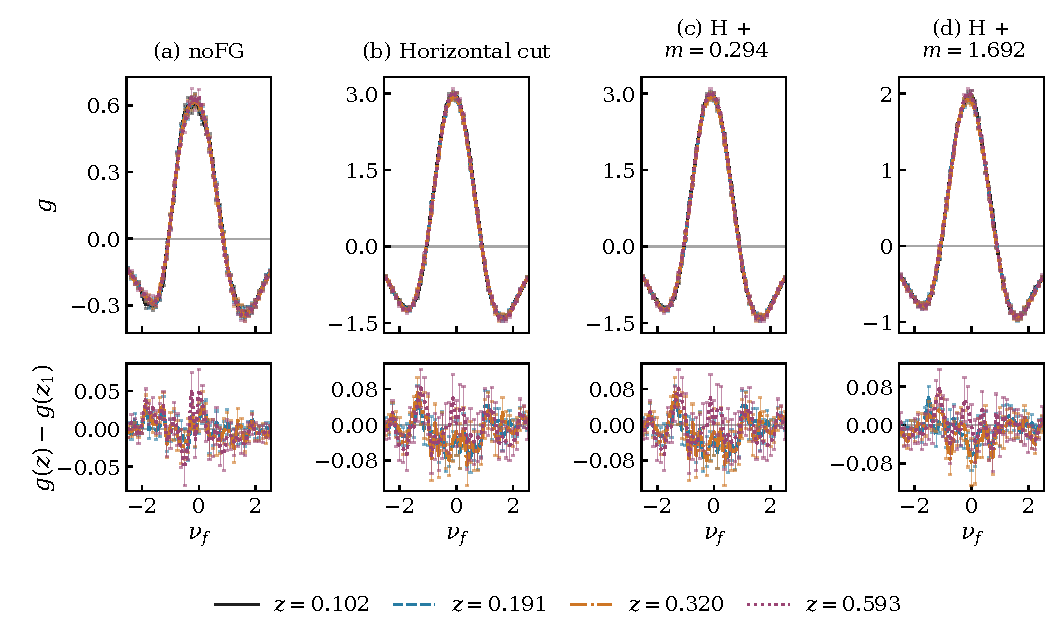
\includegraphics[width=.99\textwidth]{figures/fig__diff_redshifts.pdf}
\caption{Genus curves at the four redshifts in the simulation cosmology (top) and their differences from $z_1=0.102$ (bottom), in units of $10^{-6}h^3\mathrm{Mpc}^{-3}$.}\label{fig:redshifts}

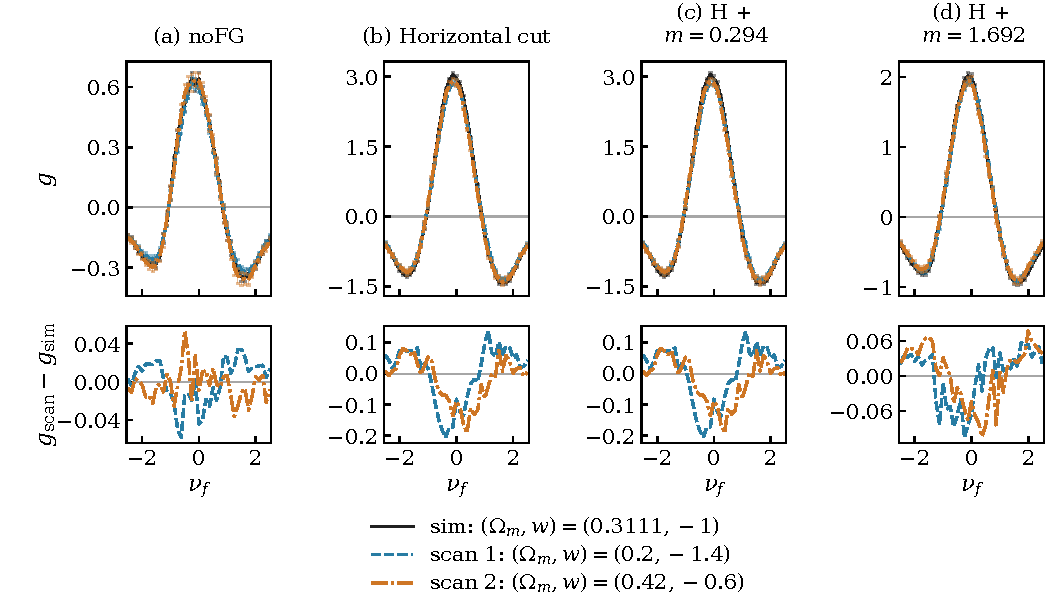
\includegraphics[width=\textwidth]{figures/fig__diff_cosmo.pdf}
\caption{Genus curves at $z=0.593$ in the simulation cosmology and two illustrative cosmologies, $(\Omega_m,w)=(0.2,-1.4)$ and $(0.42,-0.6)$ (top), and their differences from the simulation cosmology (bottom). Values are in units of $10^{-6}h^3\mathrm{Mpc}^{-3}$. The two illustrative points lie outside the 1285-point scan set.}\label{fig:cosmologies}
\end{figure*}

\begin{figure*}
\centering
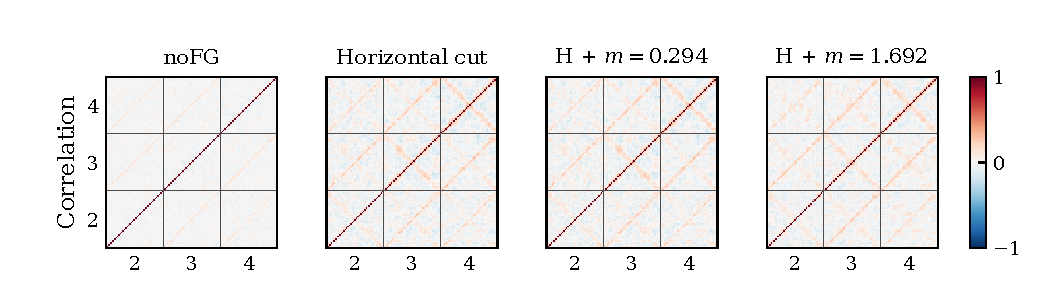
\includegraphics[width=\textwidth]{figures/fig__covmat__correlation.pdf}
\caption{Correlation matrices derived from the regularized covariance of the 123-component difference vector for the four foreground treatments. Axis numbers 2, 3 and 4 identify the redshift pairs $z_i-z_1$, with $\nu_f$ increasing from $-2.5$ to 2.5 within each block. Supplementary Fig.~S4 also shows the covariance amplitudes.}\label{fig:covariance}
\vspace{6pt}
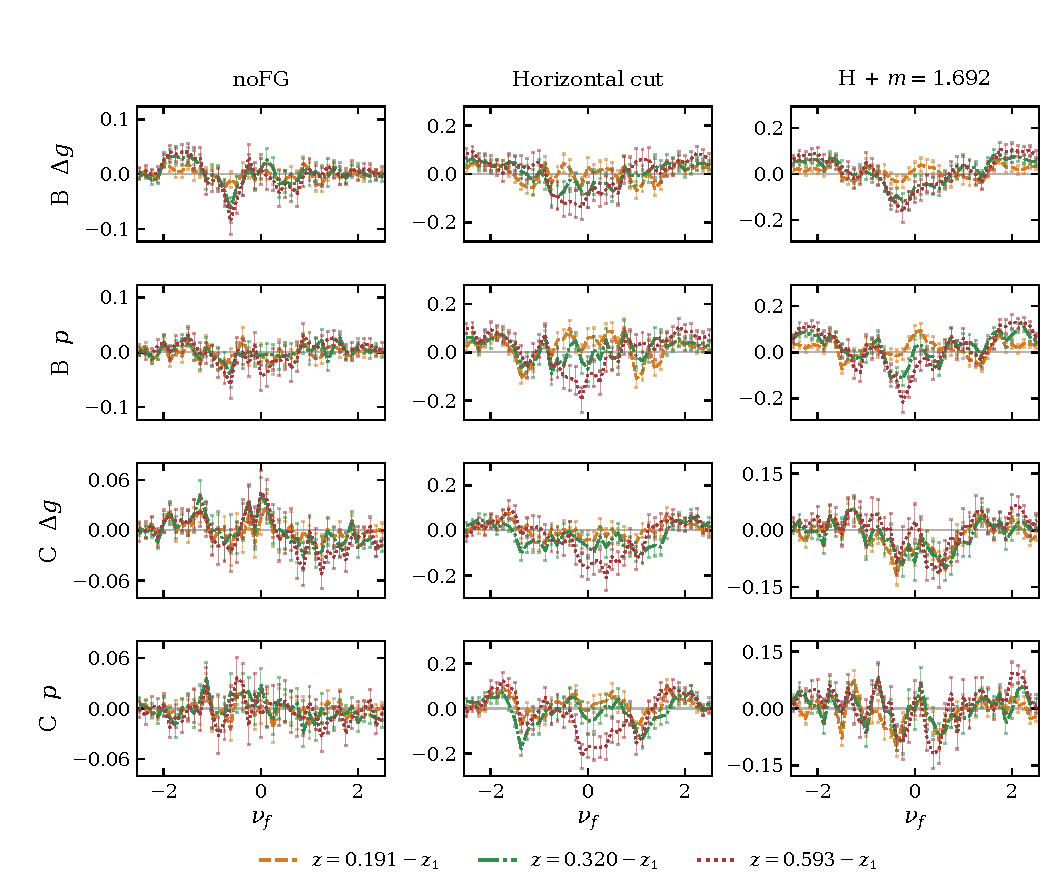
\includegraphics[width=.99\textwidth]{figures/fig__cosmo_redshift_evolution__compact.pdf}
\caption{Redshift differences $\Delta g=g(z_i)-g(z_1)$ and intrinsic-subtracted residuals $p=\Delta g-I$ for two illustrative cosmologies, B: $(\Omega_m,w)=(0.2,-1.4)$ and C: $(0.42,-0.6)$. Columns show no foreground cut, the horizontal cut and the strong wedge. Colours and line styles identify the three redshift pairs; values are in $10^{-6}h^3\mathrm{Mpc}^{-3}$. Error bars use the same fixed difference covariance as the statistic. The simulation-cosmology curves, raw genus rows and weak-wedge column are retained in Supplementary Fig.~S1.}\label{fig:evolution}
\end{figure*}

\subsection{Cosmological Constraints}\label{sec:fourcases}
We examine parameter regions conditional on the simulation, intrinsic template and idealized foreground model specified above. Here these regions describe the pipeline response; the numerical tests below limit their interpretation as cosmological constraints. Fig.~\ref{fig:fourcases} shows the smoothed regions for each redshift pair and their joint statistic. The dominant degeneracy runs towards more negative $w$ as $\Omega_m$ increases. Near the simulation cosmology, increasing $\Omega_m$ raises $E(z)$, whereas decreasing $w$ lowers the dark-energy contribution at $z>0$. Their partial compensation can produce similar expansion rates and distances over the redshift interval considered here, consistent with the observed direction. The contour orientation alone does not validate the inferred precision.

The joint regions are more localized than the individual-pair regions in Fig.~\ref{fig:fourcases}. At 68.3 per cent, the noFG joint area is 3.81 times the horizontal-cut area; the weakest wedge gives essentially the same area as the horizontal cut. Some single-pair regions and the outer joint regions reach the scan boundary, so their areas remain conditional on the sampled domain. The parameter-space smoothing is part of the definition of all areas reported in this section.

\begin{figure*}
\centering
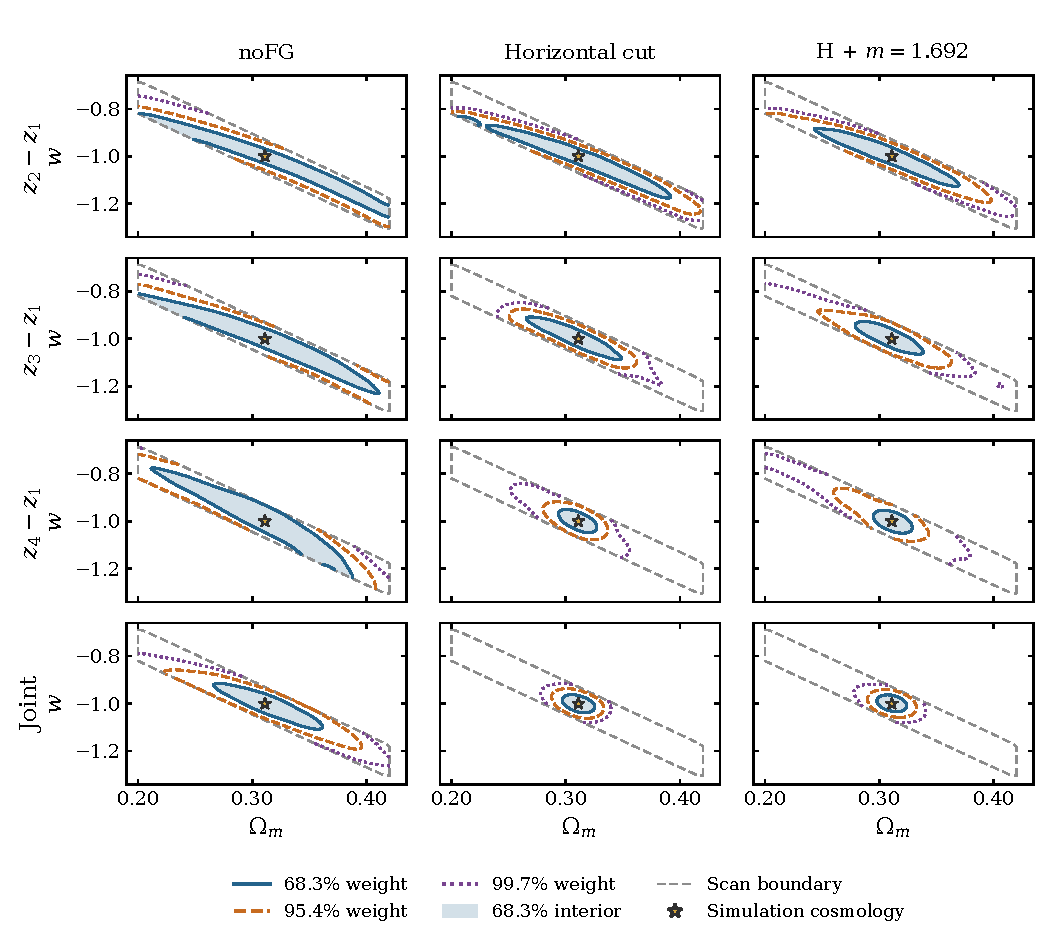
\includegraphics[width=\textwidth]{figures/fig__intrinsic_subtracted_contours__four_cases.pdf}
\caption{Smoothed parameter regions for the three redshift differences and their joint statistic in three foreground treatments. The weak-wedge case is retained in Supplementary Fig.~S2. Blue solid, orange dashed and purple dotted lines enclose 68.3, 95.4 and 99.7 per cent of the normalized weight; the 68.3 per cent interior is shaded. Grey dashed lines mark the scan boundary, and stars mark the simulation cosmology. Every panel uses the same weight interpolation, smoothing kernel and normalization domain. Common axis ranges retain boundary-reaching regions.}\label{fig:fourcases}
\end{figure*}

\subsection{Dependence on the wedge slope}\label{sec:wedgeareas}
Fig.~\ref{fig:areas} shows the joint area ratio $\mathcal R_f(m)=A_f(\mathrm{H}+m)/A_f(\mathrm{H})$ for the adopted smoothed weights, where $f$ denotes the enclosed weight fraction. Over the displayed slopes, the ratios span 0.81--1.05, 0.82--1.08 and 0.85--1.09 for $f=0.683$, 0.954 and 0.997, respectively. The variation is non-monotonic, and the smallest sampled area occurs at $m\simeq1.517$ at all three levels. At 68.3 per cent this is a 19.3 per cent reduction relative to the horizontal cut. The trend panel displays $m\le1.605$; the additional $m=1.692$ case is retained in Supplementary Table~S1 and Fig.~\ref{fig:smoothedcontours}.

\begin{figure*}
\centering
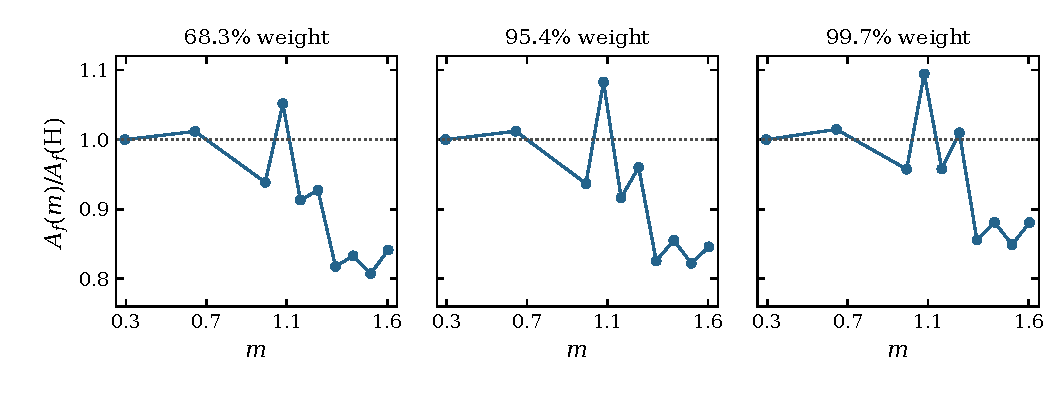
\includegraphics[width=\textwidth]{figures/fig__intrinsic_subtracted_contours__eleven_m_areas.pdf}
\caption{Joint-region areas relative to the horizontal cut for the adopted smoothed weight surface. Each panel gives one enclosed weight fraction; points are the ten sampled slopes up to $m=1.605$, and connecting lines guide the eye. Dotted lines mark unity. The trend display omits the endpoint $m=1.692$, whose result remains in Supplementary Table~S1 and Fig.~\ref{fig:smoothedcontours}.}\label{fig:areas}
\end{figure*}



Fig.~\ref{fig:smoothedcontours} compares three representative wedge cases with the horizontal-cut reference; Supplementary Fig.~S3 retains all eleven slopes. The weakest wedge almost coincides with that reference, while steeper wedges change both the area and the outer contour shape. The similar central contours and their modest area differences show that a larger removed Fourier region does not produce a monotonic change in these conditional constraints. Mode removal changes the measured genus response and its covariance weighting together; the comparison does not establish an optimal foreground cut for an observation.

\begin{figure*}
\centering
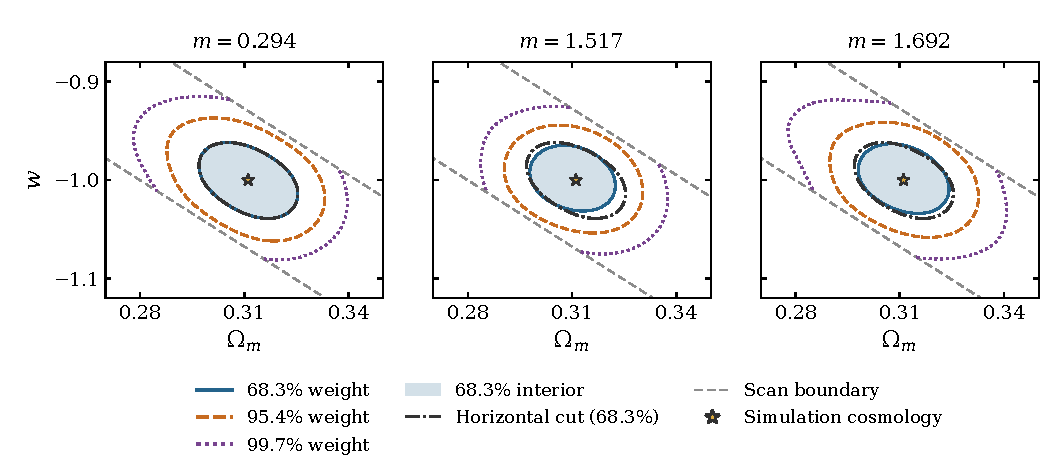
\includegraphics[width=\textwidth]{figures/fig__intrinsic_subtracted_contours__representative_smoothed.pdf}
\caption{Joint parameter regions for three representative wedge slopes, using the adopted smoothed weights. The full eleven-slope comparison is retained in Supplementary Fig.~S3. Blue solid, orange dashed and purple dotted lines enclose 68.3, 95.4 and 99.7 per cent of the weight within the common scan domain; blue shading marks the 68.3 per cent interior. The dark dash-dotted line is the horizontal-cut 68.3 per cent reference, processed with the same kernel. Grey dashed lines indicate the scan boundary, and gold stars indicate the simulation cosmology. All panels share the displayed ranges.}\label{fig:smoothedcontours}
\end{figure*}

\subsection{Numerical sensitivity of the parameter regions}\label{sec:numerics}
The parameter-area comparisons are sensitive to both field discretization and weight smoothing. In two pairs of almost identical trial cosmologies, separated by about $10^{-7}$ in their parameters, the horizontal-cut statistic jumps by 21.04 and 11.79 when an integer mesh count changes. Keeping $250^3$ cells removes these particular jumps (Table~\ref{tab:stability}). This test changes the cell size continuously with the AP-scaled box and is a diagnostic alternative to the main measurement, not an established converged estimator.

A separate 45-position line at fixed $w=-0.92451$ reveals another discontinuity even with fixed mesh counts: a discrete line-of-sight Fourier mode crosses the hard-cut boundary. The horizontal-cut statistic changes by $-23.37$ across a parameter separation of $10^{-7}$. Replacing the sharp cut by a hyperbolic-tangent transition suppresses this jump, but also changes the retained modes. Appendix~\ref{app:implementation} specifies the diagnostic filter. These examples identify two sources of numerical sensitivity; they do not establish that all residuals are numerical artifacts or that the alternative filter has converged.

\begin{table}
\centering
\caption{Changes in the horizontal-cut statistic across three close parameter pairs. The first two cross integer-mesh boundaries in the main scheme; the third crosses a hard-mask boundary in the fixed-mesh scheme. The same main covariance is used throughout.}\label{tab:stability}
\begin{tabular}{@{}lrrr@{}}\toprule
Pair & Main & Fixed mesh & Fixed + taper \\\midrule
Mesh boundary 1 & 21.037 & $-0.00181$ & $-0.000034$ \\
Mesh boundary 2 & 11.787 & $0.000015$ & $-0.00117$ \\
Mask boundary & $-0.000062$ & $-23.371$ & $-0.000021$ \\\bottomrule
\end{tabular}
\end{table}

For a matched 271-node subdomain, changing both the mesh prescription and filter changes the unsmoothed 68.3 per cent wedge-to-horizontal area ratio at $m=1.343$ from 0.497 to 1.184 with the original covariance, and to 1.220 when the tapered field has its covariance re-estimated. The regions at this level do not touch the subdomain boundary. This reversal tests robustness under different numerical and filtering choices; it does not isolate a pure discretization correction, and these subdomain values do not replace the full-scan results above.

Parameter-space smoothing produces a further change. At 68.3 per cent, it enlarges the noFG area by 2.49 and the horizontal-cut area by 6.71, changing their ratio from 10.28 to 3.81. Wedge areas increase by factors of 6.6--12.8. The smaller smoothed regions and the sampled minimum near $m=1.517$ therefore remain properties of the specified construction. They do not establish an optimal foreground cut or an improvement in observational precision.
